\documentclass{article}
\usepackage{graphicx}
\graphicspath{{images/}}
\usepackage[bottom=20mm]{geometry}
\usepackage{kotex}
\usepackage{amsmath,amssymb}
\usepackage{minted}
\usepackage{tikz}
\usepackage{lipsum}
\usepackage{siunitx}
\title{정렬 알고리즘 성능 비교}
\date{%
	2018.1 자료구조 과제 04%
%	\today%
}
\author{%
2017-12878 박승원%
}
\definecolor{mintedbackground}{rgb}{0.97,0.97,0.97}
\newmintedfile[javacode]{java}{
	bgcolor=mintedbackground,
	linenos=true,
	%	numbersep=5pt,
	tabsize=4,
	fontsize=\small,
	frame=leftline,
	% adapted from KTS 10th book
	breaklines=true,
	breakbefore={/\space\\\[\{},
	breakafter={/\space,\]\}},
	breakindent=2em,tabsize=4,
	breakaftersymbolpre={},
	breakbeforesymbolpre={},
	breakbeforesymbolpost={},
	breaksymbolleft={\tiny\ensuremath{\hookrightarrow}},
	breaksymbolright={},
}
\renewcommand{\arraystretch}{1.2}

\begin{document}
	\maketitle
	\begin{abstract}
		이 문서에서는 Bubble Sort, Insertion Sort, Heap Sort, Merge Sort,
		Quick Sort, Radix Sort와 같은 정렬 알고리즘의 동작 방식을 설명하고,
		주어진 크기의 배열을 정렬하는데에 소요되는 시간을 측정하고 분석하여
		각 알고리즘의 성능을 비교한다.
	\end{abstract}

 	\section{동작 방식}
 	
 	\subsection{Bubble Sort}
 	Bubble Sort는 배열의 모든 원소가 정렬될 때까지(line 5--13)
 	맨 앞에서부터 이웃한 두 원소를 비교(line 8)하여,
 	순서가 맞지 않을 경우 바꿔주기(line 9)를 반복하여 정렬하는 알고리즘이다.
 	
	\javacode{java-files/bubble.java}
%	\clearpage
	
	\subsection{Insertion Sort}
	Insertion Sort는 매 순간 모든 원소가 정렬된 상태를 유지하며,
	새로운 원소가 추가될 때마다 그 원소가 들어갈 자리를 찾아(line 4--11)
	insert하는 알고리즘이다.
	
	\javacode{java-files/insertion.java}
%	\clearpage
	
	\subsection{Heap Sort}
	Heap Sort는 heap이라는 자료구조를 활용한다.%
	\footnote{
		여기에서는 길이 n인 배열만을 사용하기 위해
		heap의 루트 노드의 인덱스를 0으로 두었다.
		따라서 인덱스가 $ i $인 노드의 두 자식 노드는
		인덱스가 $ 2i+1, 2i+2 $ (line 2, 3)이다.
	}
	우선, 주어진 배열을 이용하여 heap을 만들기 위해 
	자식 노드가 있는 모든 노드, 즉 $ n/2-1 $ 부터 0까지의
	인덱스를 가진 노드들 대해 \texttt{percolateDown}
	과정을 수행한다. (line 17--20)
	
	여기에서 \texttt{percolateDown} 과정은,
	한 노드의 값이 그의 자식노드들 중 큰 값(line 5--8)보다
	작을 경우 둘의 위치를 바꿔주기를 반복(line 9--12)하는 방식으로
	heap의 성질을 만족시키기 위해
	삽입/변경된 특정 노드를 heap의 아래쪽으로 내려보내는 과정이다.
	
	그 다음, heap의 루트 노드를 가장 마지막 인덱스의 원소와 바꾼다. (line 24)
	그 루트 노드에 있던 값은 이제까지 다룬 heap의 최대 원소이므로 더 이상
	다루지 않는다.
	이제 가장 마지막 인덱스에 있다가 루트 노드로 올라온 원소를 \texttt{percolateDown}
	해주면 다시 heap이 되고, 여기에서 또 다시 루트 노드를 빼가기를 반복하면
	배열의 모든 원소가 정렬된다.

	\javacode{java-files/heap.java}
%	\clearpage
	
	\subsection{Merge Sort}
	Merge Sort에서는 배열의 크기가 1이 될 때까지 이등분(line 5, 6)하여 각각을 정렬하고,
	그 둘을 정렬된 배열로 병합하는 분할정복 알고리즘이다.
	
	두 배열의 맨 앞의 원소들을 비교하여 작은 값을 병합될 임시 배열에 넣고,
	이를 하나의 배열이 빌 때까지 반복한다.
	하나의 배열이 비고 나면 다른 한 배열에 남아있는 모든 원소를 임시 배열에 넣어주면
	임시 배열은 두 배열을 병합한, 정렬된 배열이 된다.
	
	\javacode{java-files/merge.java}
%	\clearpage
	
	\subsection{Quick Sort}
	Quick Sort에서는 배열의 임의의 위치에 있는 원소 하나%
	\footnote{여기에서는 맨 뒤의 원소를 사용하고 있다: line 2}를 기준으로 삼아,
	배열을 그 기준보다 작은 원소들 / 큰 원소들로 이루어진 두 개의 배열로 나누기를
	배열의 크기가 1이 될 때까지 반복한다.
	
	아래의 코드에서 \texttt{partition} 함수는 주어진 구간의 부분배열에 대해
	기준점보다 작은 원소들을 앞쪽으로, 큰 원소들을 뒤쪽으로 배치하고
	둘의 구분 지점을 \texttt{int}형으로 리턴하는 함수다.
	
	
	\javacode{java-files/quick.java}
%	\clearpage
	
	\subsection{Radix Sort}
	Radix Sort는 정수들로 이루어진 배열에 대해서만 사용할 수 있는 정렬 알고리즘이다.
	배열의 원소들을 4진법으로 나타내었을 때, 가장 작은 자리수에 대해 값이 0, 1, 2, 3인
	원소들을 하나씩 각각 임시 배열 \texttt{bucket}에 넣는다. 그 후 각각의 \texttt{bucket}에서
	모든 원소들을 다시 원래의 배열에 넣고, 이를 더 큰 자리수에 대해 계속해서 반복하면 된다.
	
	주어진 조건에서는 수가 \texttt{int}형으로 주어지기 때문에, 음의 값을 처리하기 위해
	모든 배열에 $ 2^{31} $을 더하고, \texttt{Long}형으로 수들을 다뤘다.
	

	\javacode{java-files/radix.java}
	\clearpage
	
	\section{동작 시간 분석}
	\subsection{시간복잡도 분석}
	이 문서에서 다루는 정렬 알고리즘의 시간복잡도와,
	in-place 소팅 여부는 표 \ref{tab:bigo}\와 같이 나타내어진다.
	
	\begin{table}[h]
		\centering
		\begin{tabular}{|l|c|c|c|c|}
			\hline
			Algorithm & Best-case & Average-case & Worst-case & In-place? \\
			\hline
			\textbf{B}ubble Sort & $ O(n) $ & $ O(n^{2}) $ & $ O(n^{2}) $ & O \\
			\hline
			\textbf{I}nsertion Sort & $ O(n) $ & $ O(n^{2}) $ & $ O(n^{2}) $ & O \\
			\hline
			\textbf{H}eap Sort & $ O(n\log{n}) $ & $ O(n\log{n}) $ & $ O(n\log{n}) $ & O \\
			\hline
			\textbf{M}erge Sort & $ O(n\log{n}) $ & $ O(n\log{n}) $ & $ O(n\log{n}) $ & X \\
			\hline
			\textbf{Q}uick Sort & $ O(n\log{n}) $ & $ O(n\log{n}) $ & $ O(n^{2}) $ & X \\
			\hline
			\textbf{R}adix Sort & $ O(n) $ & $ O(n) $ & $ O(n) $ & X \\
			\hline
		\end{tabular}
		\caption{%
			정렬 알고리즘의 시간복잡도.
			$ n $은 정렬할 배열의 크기이다.
		}
		\label{tab:bigo}
	\end{table}

	\subsection{수행시간 측정 및 분석}
	앞서 살펴본 알고리즘의 시간복잡도를 확인하기 위해,
	$ -10^{9} $ 이상 $ 10^{9} $ 이하의 랜덤 수들을 이용하여
	크기가 $ n $인 배열을 만들고, 각각의 알고리즘을 사용했을 때 정렬하는 데에 소요되는 시간을
	측정했다.
	
	\textbf{앞으로 등장하는 모든 그래프에서, 따로 명시하지 않는 한 가로축은 정렬하는 배열의 크기 $ n $을,
	세로축은 수행시간(\si{\milli\second})을 뜻한다.}
	
	수행 시간이 \SI{100000}{\milli\second}를 넘어가지 않는 한도 내에서,
	$ n $을 10부터 $ 10^{7} $까지 변화시켜가며 수행시간을 측정한 결과
	그림 \ref{fig:overall}\와 같았고, 이를 로그 스케일로 나타낸 결과
	그림 \ref{fig:logarithmic}\와 같았다.
	
	전체적으로 정렬 속도는
	\textbf{Quick $ > $ Merge $ > $ Heap $ > $ Radix $ > $ Insertion $ > $ Bubble}와 같았다.
	Radix Sort가 $ O(n) $ 정렬임에도 불구하고 $ O(n\log{n}) $ 정렬 알고리즘에 비해
	느렸던 것은, 음수를 처리하는 과정에서 $ 2^{31} $을 더했고,
	bucket을 4개만 사용했기 때문에 상수최적화가 충분히 되지 않았기 때문일 것이다.
	또한, Heap Sort와 Bubble Sort가 같은 시간복잡도의 알고리즘에 비해 느렸던 것은
	불필요한 swap이 많았기 떄문일 것이다.
	
	\begin{figure}[h]
		\centering
		\begin{minipage}{0.45\textwidth}
			\centering
			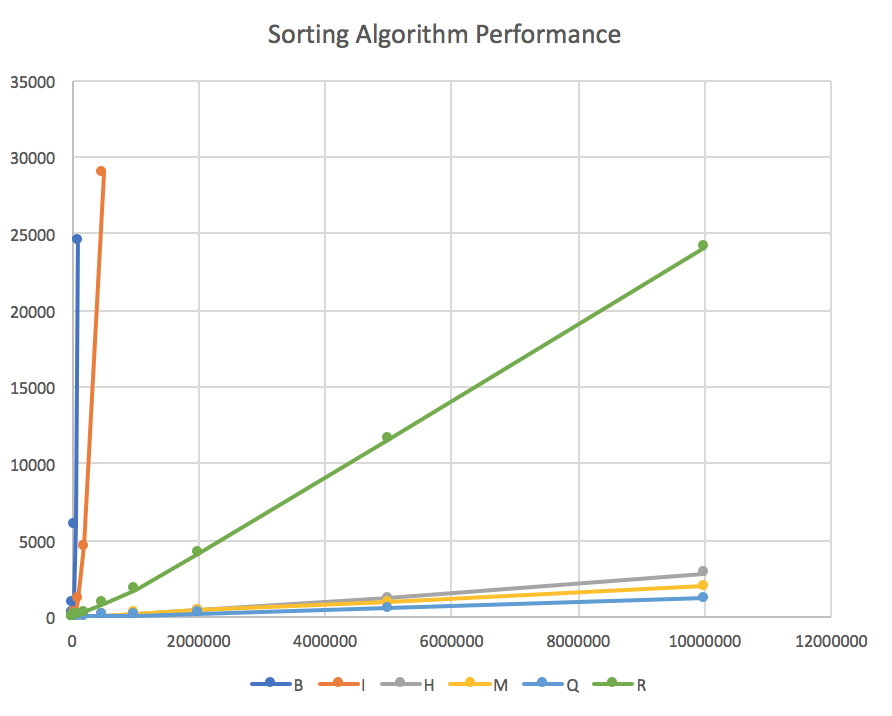
\includegraphics[width=\textwidth]{overall.png}
			\caption{알고리즘의 수행 시간.}
			\label{fig:overall}
		\end{minipage}
		\begin{minipage}{0.45\textwidth}
			\centering
			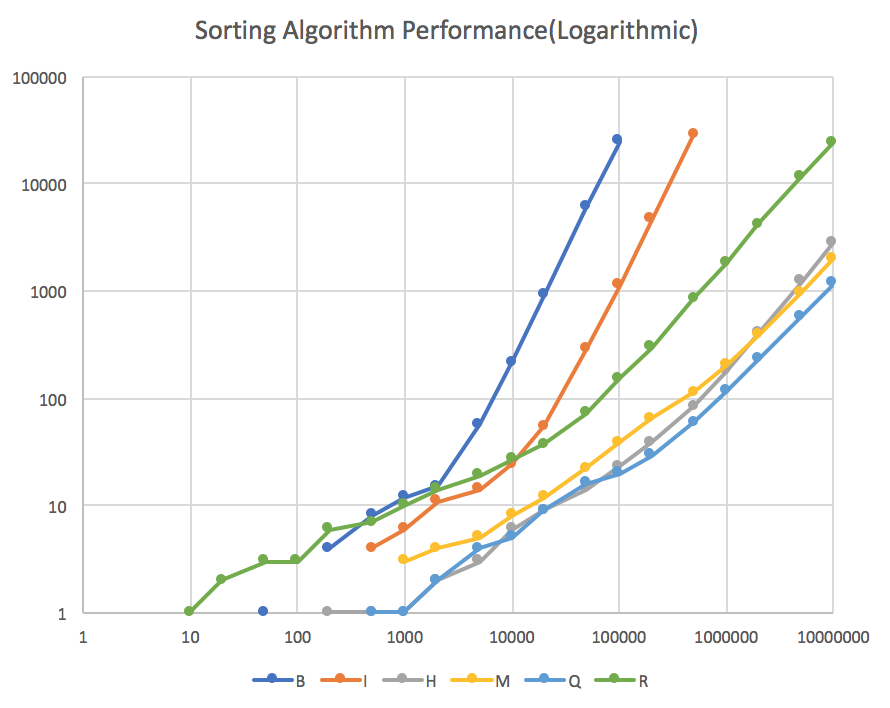
\includegraphics[width=\textwidth]{logarithmic.png}
			\caption{로그 스케일로 나타낸 그림 \ref{fig:overall}.}
			\label{fig:logarithmic}
		\end{minipage}
	\end{figure}
	\clearpage
	평균 시간복잡도가 $ O(n^{2}) $인 Bubble Sort, Insertion Sort에 대해
	$ n $에 따른 수행시간 변화를 2차다항식에 fitting한 결과
	그림 \ref{fig:bubble}, \ref{fig:insertion}\와 같이 잘 맞음을 확인할 수 있었다.
	또한, 시간복잡도가 $ O(n^{2}) $으로 동일하지만
	평균적으로 Bubble Sort가 Insertion Sort보다 느림을 확인할 수 있었다.
	\begin{figure}[h]
		\centering
		\hfill
		\begin{minipage}{0.45\textwidth}
			\centering
			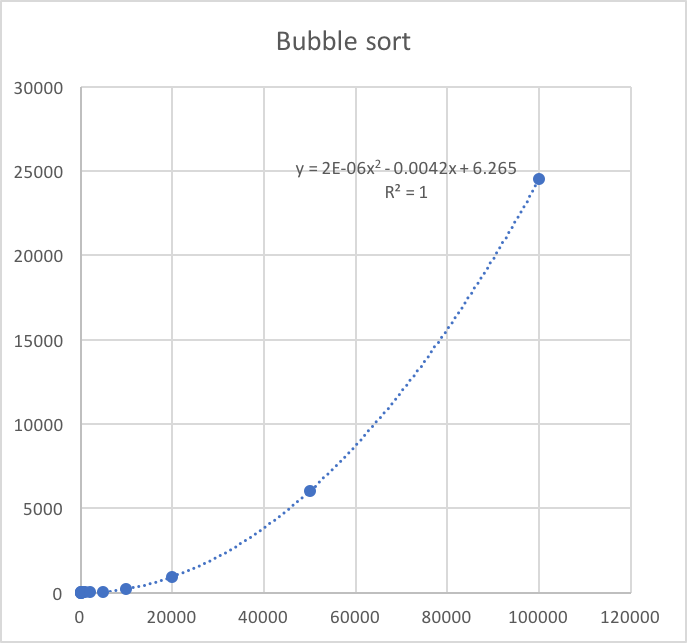
\includegraphics[width=0.9\textwidth]{B.png}
			\caption{Bubble Sort의 수행 시간.}
			\label{fig:bubble}
		\end{minipage}
		\hfill
		\begin{minipage}{0.45\textwidth}
			\centering
			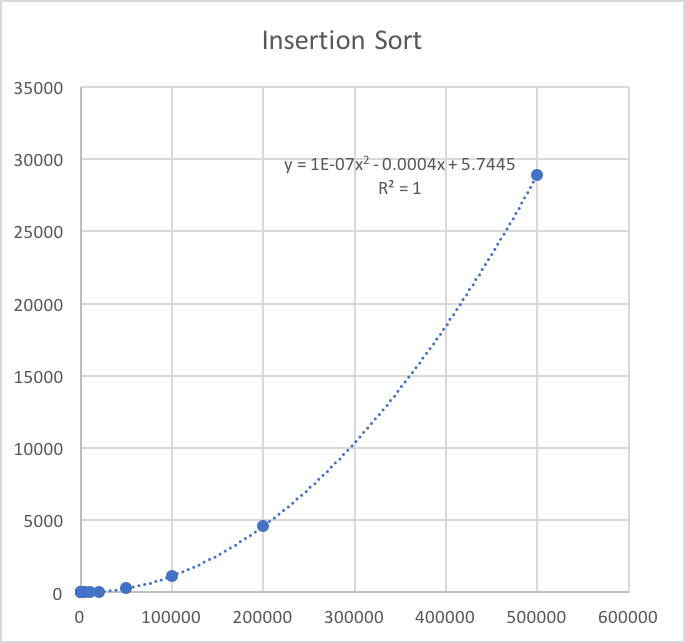
\includegraphics[width=0.9\textwidth]{I.png}
			\caption{Insertion Sort의 수행 시간.}
			\label{fig:insertion}
		\end{minipage}
		\hfill
	\end{figure}
	\vfill
	평균 시간복잡도가 $ O(n\log{n}) $인 Heap Sort, Merge Sort, Quick Sort에
	대해서는 $ n $에 대한 수행시간 변화가 그림 \ref{fig:hmq}\와 같이 나타났다.
	시간복잡도는 모두 동일하지만 평균적으로 Quick Sort가 가장 빠르고,
	그 다음 Merge Sort가 빨랐으며, Heap Sort가 가장 느림을 관찰할 수 있었다.
	\begin{figure}[h]
		\centering
		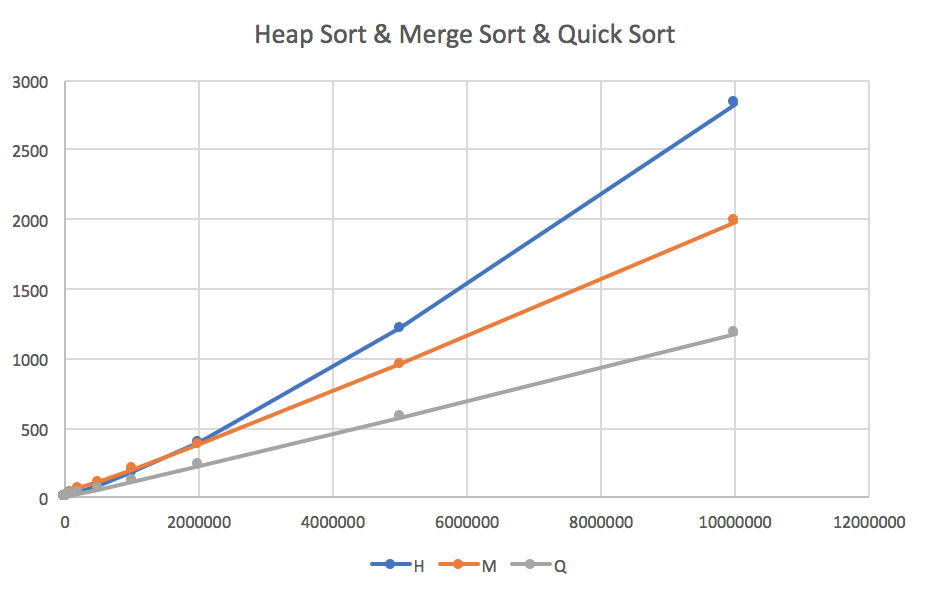
\includegraphics[width=0.7\textwidth]{HMQ.png}
		\caption{Heap Sort, Merge Sort, Quick Sort의 수행 시간.}
		\label{fig:hmq}
	\end{figure}
	\vfill

	\clearpage
	
	마지막으로, 평균 시간복잡도가 $ O(n) $인 Radix Sort에 대해
	$ n $에 대한 수행시간 변화를 그리고
	선형회귀를 한 결과, 그림 \ref{fig:radix}\와 같이
	선형적으로 변화하는 것을 확인할 수 있었다.
	\begin{figure}[h]
		\centering
		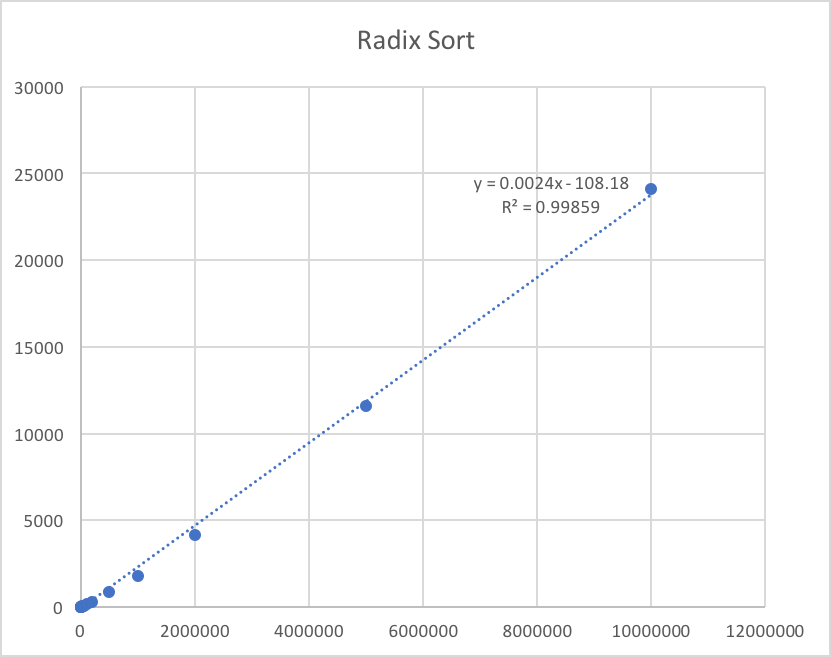
\includegraphics[width=0.7\textwidth]{R.png}
		\caption{Radix Sort의 수행 시간.}
		\label{fig:radix}
	\end{figure}
\end{document}